%% main.tex
%% Created by Ayan Chakrabarti from the IEEE bare_jrnl_compsoc.tex file.
%% Modified by Ioannis Gkioulekas.
%%
%% bare_jrnl_compsoc.tex
%% V1.4b
%% 2015/08/26
%% by Michael Shell
%% See:
%% http://www.michaelshell.org/
%% for current contact information.
%%
%% This is a skeleton file demonstrating the use of IEEEtran.cls
%% (requires IEEEtran.cls version 1.8b or later) with an IEEE
%% Computer Society journal paper.
%%
%% Support sites:
%% http://www.michaelshell.org/tex/ieeetran/
%% http://www.ctan.org/pkg/ieeetran
%% and
%% http://www.ieee.org/

%%*************************************************************************
%% Legal Notice:
%% This code is offered as-is without any warranty either expressed or
%% implied; without even the implied warranty of MERCHANTABILITY or
%% FITNESS FOR A PARTICULAR PURPOSE! 
%% User assumes all risk.
%% In no event shall the IEEE or any contributor to this code be liable for
%% any damages or losses, including, but not limited to, incidental,
%% consequential, or any other damages, resulting from the use or misuse
%% of any information contained here.
%%
%% All comments are the opinions of their respective authors and are not
%% necessarily endorsed by the IEEE.
%%
%% This work is distributed under the LaTeX Project Public License (LPPL)
%% ( http://www.latex-project.org/ ) version 1.3, and may be freely used,
%% distributed and modified. A copy of the LPPL, version 1.3, is included
%% in the base LaTeX documentation of all distributions of LaTeX released
%% 2003/12/01 or later.
%% Retain all contribution notices and credits.
%% ** Modified files should be clearly indicated as such, including  **
%% ** renaming them and changing author support contact information. **
%%*************************************************************************


\documentclass[10pt,journal,compsoc]{IEEEtran}
\newif\ifpeerreview

%%% Important: for camera ready submissions, replace the following line
%%% with \peerreviewfalse
\peerreviewfalse


\usepackage[nocompress]{cite}
\usepackage{url}
\usepackage{amsmath,amssymb,graphicx}

\usepackage{lipsum} % Only used to generate random text.


\usepackage[switch]{lineno}

\usepackage{booktabs}
\usepackage{siunitx}
\usepackage{xcolor}
\usepackage[hidelinks]{hyperref}
\usepackage[capitalise]{cleveref}

% Run-in headings (\paragraph): unnumbered and bold. The class numbers them (2.0.0.1) and adds a colon,
% which doubled our own full stops ("Coded exposure.:"); our titles end in their own punctuation.
\setcounter{secnumdepth}{3}
\makeatletter
\def\@IEEEsectpunct{\ }
\def\paragraph{\@startsection{paragraph}{4}{2\parindent}{-0ex plus -0.1ex minus -0.1ex}{0ex}{\normalfont\normalsize\bfseries}}
\makeatother

% Writing aids. Set \showtodostrue to \showtodosfalse before submitting: every TODO vanishes,
% and every \placeholder figure still shows as a box, so nothing unfinished can slip through.
\newif\ifshowtodos \showtodostrue
\newcommand{\TODO}[1]{\ifshowtodos{\color{red}\textbf{[TODO:} #1\textbf{]}}\fi}
\newcommand{\placeholder}[2][\linewidth]{%   \placeholder[width]{what goes here}
  \fbox{\parbox[c][0.55#1][c]{\dimexpr#1-2\fboxsep-2\fboxrule}{\centering\small\color{gray}#2}}}
\newcommand{\X}{\textcolor{red}{\textbf{XX}}}  % a number still to measure

\graphicspath{{figures/}}
% Let more floats share a page, so figures stay near their first mention instead of queueing
% behind each other until after the references.
\renewcommand{\topfraction}{0.9}\renewcommand{\dbltopfraction}{0.9}
\renewcommand{\bottomfraction}{0.8}\renewcommand{\textfraction}{0.07}
\renewcommand{\floatpagefraction}{0.8}\renewcommand{\dblfloatpagefraction}{0.8}
\setcounter{topnumber}{3}\setcounter{bottomnumber}{2}\setcounter{totalnumber}{5}\setcounter{dbltopnumber}{2}
% Every measured or simulated number in the text is a macro from this file, written by
% figures/make_figures.py. A missing macro stops the build, so a stale number cannot slip in.
% written by make_figures.py: do not edit by hand
\newcommand{\boxMinMTF}{0}
\newcommand{\gainBlurOne}{25}
\newcommand{\gainBlurThree}{101}
\newcommand{\gainBlurTwo}{51}
\newcommand{\gainCodedFullOne}{36.9}
\newcommand{\gainCodedFullThree}{35.5}
\newcommand{\gainCodedFullTwo}{36.1}
\newcommand{\gainCodedTenthOne}{30.4}
\newcommand{\gainCodedTenthThree}{28.9}
\newcommand{\gainCodedTenthTwo}{30.3}
\newcommand{\gainShortFullOne}{34.4}
\newcommand{\gainShortFullThree}{28.5}
\newcommand{\gainShortFullTwo}{32.3}
\newcommand{\gainShortTenthOne}{25.5}
\newcommand{\gainShortTenthThree}{24.9}
\newcommand{\gainShortTenthTwo}{25.3}
\newcommand{\gainSteadyFullOne}{35.9}
\newcommand{\gainSteadyFullThree}{27.0}
\newcommand{\gainSteadyFullTwo}{31.0}
\newcommand{\gainSteadyTenthOne}{29.8}
\newcommand{\gainSteadyTenthThree}{23.5}
\newcommand{\gainSteadyTenthTwo}{26.3}
\newcommand{\psnrConstLetters}{40.5}
\newcommand{\psnrConstTex}{36.1}
\newcommand{\psnrGsLetters}{43.7}
\newcommand{\psnrGsTex}{36.9}
\newcommand{\psnrRsFrameLetters}{40.1}
\newcommand{\psnrRsFrameTex}{36.4}
\newcommand{\psnrRsRowLetters}{43.5}
\newcommand{\psnrRsRowTex}{36.8}
\newcommand{\psnrShortLetters}{24.4}
\newcommand{\psnrShortTex}{26.8}
\newcommand{\raskarMinMTF}{0.051}
\newcommand{\realBitMs}{62.5}
\newcommand{\realBits}{304}
\newcommand{\realLateBits}{1}
\newcommand{\realMaxLateMs}{7.1}
\newcommand{\realMaxLatePct}{11}
\newcommand{\realRuns}{19}
\newcommand{\realWithinOneMs}{298}
\newcommand{\rigBandGapMax}{8.1}
\newcommand{\rigBandGapMean}{5.6}
\newcommand{\rigBandGapMin}{1.9}
\newcommand{\rigBandsUsed}{7}
\newcommand{\rigBits}{16}
\newcommand{\rigCaptures}{65}
\newcommand{\rigCardCoded}{24.0}
\newcommand{\rigCardRsCoded}{16.9}
\newcommand{\rigCardRsSteady}{9.5}
\newcommand{\rigCardSpeed}{8}
\newcommand{\rigCardSteady}{16.5}
\newcommand{\rigCardsAll}{65}
\newcommand{\rigCardsRead}{65}
\newcommand{\rigCodeMs}{66.7}
\newcommand{\rigCodeS}{1.067}
\newcommand{\rigCodedEight}{24.0}
\newcommand{\rigCodedEightN}{11}
\newcommand{\rigCodedEightSd}{2.1}
\newcommand{\rigCodedFive}{23.3}
\newcommand{\rigCodedFiveN}{12}
\newcommand{\rigCodedFiveSd}{1.5}
\newcommand{\rigCodedThree}{25.7}
\newcommand{\rigCodedThreeN}{12}
\newcommand{\rigCodedThreeSd}{2.8}
\newcommand{\rigFlipped}{0}
\newcommand{\rigGapMax}{7.1}
\newcommand{\rigGapMin}{5.6}
\newcommand{\rigMarginMin}{1.2}
\newcommand{\rigMinMTF}{0.148}
\newcommand{\rigOctTwentySix}{23.4}
\newcommand{\rigOctTwentySixMarginMin}{1.0}
\newcommand{\rigOctTwentySixN}{11}
\newcommand{\rigOctTwentySixSd}{3.0}
\newcommand{\rigReadCodedEight}{91}
\newcommand{\rigReadCodedEightN}{11}
\newcommand{\rigReadCodedFive}{100}
\newcommand{\rigReadCodedFiveN}{12}
\newcommand{\rigReadCodedThree}{100}
\newcommand{\rigReadCodedThreeN}{12}
\newcommand{\rigReadRawCoded}{0}
\newcommand{\rigReadRawRsCoded}{0}
\newcommand{\rigReadRawRsSteady}{0}
\newcommand{\rigReadRawSteady}{0}
\newcommand{\rigReadRsCodedEight}{60}
\newcommand{\rigReadRsCodedEightN}{10}
\newcommand{\rigReadRsCodedFive}{80}
\newcommand{\rigReadRsCodedFiveN}{10}
\newcommand{\rigReadRsCodedThree}{100}
\newcommand{\rigReadRsCodedThreeN}{10}
\newcommand{\rigReadRsSteadyEight}{20}
\newcommand{\rigReadRsSteadyEightN}{10}
\newcommand{\rigReadRsSteadyFive}{44}
\newcommand{\rigReadRsSteadyFiveN}{9}
\newcommand{\rigReadRsSteadyThree}{60}
\newcommand{\rigReadRsSteadyThreeN}{10}
\newcommand{\rigReadSteadyEight}{0}
\newcommand{\rigReadSteadyEightN}{10}
\newcommand{\rigReadSteadyFive}{90}
\newcommand{\rigReadSteadyFiveN}{10}
\newcommand{\rigReadSteadyThree}{90}
\newcommand{\rigReadSteadyThreeN}{10}
\newcommand{\rigRsBandsUsed}{7}
\newcommand{\rigRsCaptures}{59}
\newcommand{\rigRsCardsAll}{59}
\newcommand{\rigRsCardsRead}{59}
\newcommand{\rigRsCodedEight}{18.0}
\newcommand{\rigRsCodedEightN}{10}
\newcommand{\rigRsCodedEightSd}{1.8}
\newcommand{\rigRsCodedFive}{18.0}
\newcommand{\rigRsCodedFiveN}{10}
\newcommand{\rigRsCodedFiveSd}{0.6}
\newcommand{\rigRsCodedThree}{18.1}
\newcommand{\rigRsCodedThreeN}{10}
\newcommand{\rigRsCodedThreeSd}{0.9}
\newcommand{\rigRsFlipped}{0}
\newcommand{\rigRsGapMax}{8.0}
\newcommand{\rigRsGapMin}{6.4}
\newcommand{\rigRsMarginMin}{1.3}
\newcommand{\rigRsSteadyEight}{10.3}
\newcommand{\rigRsSteadyEightN}{10}
\newcommand{\rigRsSteadyEightSd}{1.6}
\newcommand{\rigRsSteadyFive}{10.1}
\newcommand{\rigRsSteadyFiveN}{9}
\newcommand{\rigRsSteadyFiveSd}{1.1}
\newcommand{\rigRsSteadyThree}{11.7}
\newcommand{\rigRsSteadyThreeN}{10}
\newcommand{\rigRsSteadyThreeSd}{0.9}
\newcommand{\rigSpeedAllCoded}{35}
\newcommand{\rigSpeedAllRsCoded}{30}
\newcommand{\rigSpeedAllRsSteady}{29}
\newcommand{\rigSpeedAllSteady}{30}
\newcommand{\rigSpeedCodedEight}{-1.2}
\newcommand{\rigSpeedCodedEightSd}{1.1}
\newcommand{\rigSpeedCodedFive}{-1.3}
\newcommand{\rigSpeedCodedFiveSd}{1.0}
\newcommand{\rigSpeedCodedThree}{-2.3}
\newcommand{\rigSpeedCodedThreeSd}{2.2}
\newcommand{\rigSpeedEdgeCoded}{0}
\newcommand{\rigSpeedEdgeRsCoded}{0}
\newcommand{\rigSpeedEdgeRsSteady}{0}
\newcommand{\rigSpeedEdgeSteady}{0}
\newcommand{\rigSpeedRsCodedEight}{-1.5}
\newcommand{\rigSpeedRsCodedEightSd}{1.4}
\newcommand{\rigSpeedRsCodedFive}{-0.1}
\newcommand{\rigSpeedRsCodedFiveSd}{1.7}
\newcommand{\rigSpeedRsCodedThree}{-1.0}
\newcommand{\rigSpeedRsCodedThreeSd}{1.6}
\newcommand{\rigSpeedRsSteadyEight}{+1.7}
\newcommand{\rigSpeedRsSteadyEightSd}{1.5}
\newcommand{\rigSpeedRsSteadyFive}{+2.5}
\newcommand{\rigSpeedRsSteadyFiveSd}{1.0}
\newcommand{\rigSpeedRsSteadyThree}{+3.0}
\newcommand{\rigSpeedRsSteadyThreeSd}{1.3}
\newcommand{\rigSpeedSteadyEight}{-5.8}
\newcommand{\rigSpeedSteadyEightSd}{1.4}
\newcommand{\rigSpeedSteadyFive}{-4.1}
\newcommand{\rigSpeedSteadyFiveSd}{1.7}
\newcommand{\rigSpeedSteadyThree}{-3.9}
\newcommand{\rigSpeedSteadyThreeSd}{1.6}
\newcommand{\rigSpeedWithinCoded}{34}
\newcommand{\rigSpeedWithinRsCoded}{30}
\newcommand{\rigSpeedWithinRsSteady}{27}
\newcommand{\rigSpeedWithinSteady}{17}
\newcommand{\rigSpeedWorstCoded}{8.0}
\newcommand{\rigSpeedWorstRsCoded}{4.3}
\newcommand{\rigSpeedWorstRsSteady}{5.7}
\newcommand{\rigSpeedWorstSteady}{8.7}
\newcommand{\rigSteadyEight}{16.9}
\newcommand{\rigSteadyEightN}{10}
\newcommand{\rigSteadyEightSd}{1.7}
\newcommand{\rigSteadyFive}{17.6}
\newcommand{\rigSteadyFiveN}{10}
\newcommand{\rigSteadyFiveSd}{2.0}
\newcommand{\rigSteadyThree}{18.9}
\newcommand{\rigSteadyThreeN}{10}
\newcommand{\rigSteadyThreeSd}{3.0}
\newcommand{\rowsMaxGapA}{1.2}
\newcommand{\rowsMaxGapB}{0.5}
\newcommand{\rowsMaxMeanGapA}{0.3}
\newcommand{\rowsMaxMeanGapB}{0.2}
\newcommand{\rowsShortDropA}{14.1}
\newcommand{\rowsShortDropB}{6.7}
\newcommand{\rowsShortFrameMeanA}{26.3}
\newcommand{\rowsShortFrameMeanB}{33.0}
\newcommand{\rowsShortFrameWorstA}{19.0}
\newcommand{\rowsShortFrameWorstB}{28.7}
\newcommand{\rowsShortGlobalMeanA}{40.4}
\newcommand{\rowsShortGlobalMeanB}{39.8}
\newcommand{\rowsShortRowMeanA}{40.0}
\newcommand{\rowsShortRowMeanB}{39.7}
\newcommand{\speedErrLetters}{0.0}
\newcommand{\speedErrSignedLetters}{+0.0}
\newcommand{\speedErrSignedTex}{+0.2}
\newcommand{\speedErrTex}{0.2}
\newcommand{\ssimConstLetters}{0.998}
\newcommand{\ssimConstTex}{0.979}
\newcommand{\ssimGsLetters}{0.999}
\newcommand{\ssimGsTex}{0.979}
\newcommand{\ssimRsFrameLetters}{0.997}
\newcommand{\ssimRsFrameTex}{0.978}
\newcommand{\ssimRsRowLetters}{0.999}
\newcommand{\ssimRsRowTex}{0.979}
\newcommand{\ssimShortLetters}{0.794}
\newcommand{\ssimShortTex}{0.868}
\newcommand{\tikConstLetters}{26.4}
\newcommand{\tikConstTex}{27.8}
\newcommand{\tikGsLetters}{27.6}
\newcommand{\tikGsTex}{28.8}
\newcommand{\tikRsFrameLetters}{27.1}
\newcommand{\tikRsFrameTex}{28.5}
\newcommand{\tikRsRowLetters}{27.3}
\newcommand{\tikRsRowTex}{28.5}
\newcommand{\tikSsimConstLetters}{0.889}
\newcommand{\tikSsimConstTex}{0.918}
\newcommand{\tikSsimGsLetters}{0.875}
\newcommand{\tikSsimGsTex}{0.920}
\newcommand{\tikSsimRsFrameLetters}{0.871}
\newcommand{\tikSsimRsFrameTex}{0.916}
\newcommand{\tikSsimRsRowLetters}{0.871}
\newcommand{\tikSsimRsRowTex}{0.916}



% Insert your paper ID and information below
\newcommand{\paperID}{XXXX}

% Enter your paper title below
\title{Coded Illumination for Motion Deblurring:\\
  Global Shutter versus Rolling Shutter}

% Enter your author information before
% Note this is only necessary for the camera review. Submissions are anonymized.
\author{
  Jack Thompson \quad Oliver Turner \quad Krish Singh \quad Daniel Chung \quad Ben Ritchie\\
  {\small Code and data: \url{https://github.com/chung-811/mech5720-2026-codedillumination}}   
}


\begin{document}

\IEEEtitleabstractindextext{%
\begin{abstract}
% Brief: whole report, no jargon, avoid acronyms, NO citations, include specific key numbers.
\begin{abstract}
Photographs of moving objects blur, and a shorter exposure trades the blur for darkness and noise.
We built a camera system that avoids this trade-off without modifying the camera: a computer monitor
beside it flashes a designed on/off pattern during one long exposure, which makes the blur
reversible. A fan with letters on its blades, driven by a stepper motor at a known speed, is the
subject. We compare a camera that exposes every row at once with one that exposes row by row,
corrected either once per image or row by row. In simulation, our reconstruction recovers a textured
blade to \psnrGsTex~dB against the stopped fan; correcting row by row matches the all-at-once camera
to within \rowsMaxMeanGapA~dB on average over the image; and the fan's speed is recovered from a single
photograph to within \speedErrTex\%. On the real rig, the monitor showed the pattern to within one
millisecond for \realWithinOneMs~of \realBits~flashes, and with the all-at-once camera at 3 to 8
revolutions per minute the reconstructions score \rigGapMin~to \rigGapMax~dB higher than steady light
reconstructed the same way; the row-by-row camera, which images the fan larger, scores lower but keeps
a \rigRsGapMin~to \rigRsGapMax~dB lead. At 8 revolutions per minute a character reader reads
\rigReadCodedEight\% of the letters after reconstruction with coded light and \rigReadSteadyEight\%
with steady light, and the speed measured from the blur is within 5\% of the set speed on
\rigSpeedWithinCoded~of \rigSpeedAllCoded~and \rigSpeedWithinRsCoded~of \rigSpeedAllRsCoded~coded
photographs from the two cameras.
\end{abstract}

\end{abstract}
}


% Make Title
\ifpeerreview
\linenumbers \linenumbersep 15pt\relax 
\author{Paper ID \paperID\IEEEcompsocitemizethanks{\IEEEcompsocthanksitem This paper is under review for ICCP 2026 and the PAMI special issue on computational photography. Do not distribute.}}
\markboth{Anonymous ICCP 2026 submission ID \paperID}%
{}
\fi
\maketitle



% The first section title should be wrapped inside a \IEEEraisesectionheading as follows.
\IEEEraisesectionheading{
  \section{Introduction}\label{sec:intro}
}
\IEEEPARstart{P}{HOTOGRAPHING} % Brief: motivation (why anyone should care), principle of operation at a high level, what is new.
% Journalistic style: the first sentence of each paragraph says what it is about.

\begin{figure}[b]
  \centering
  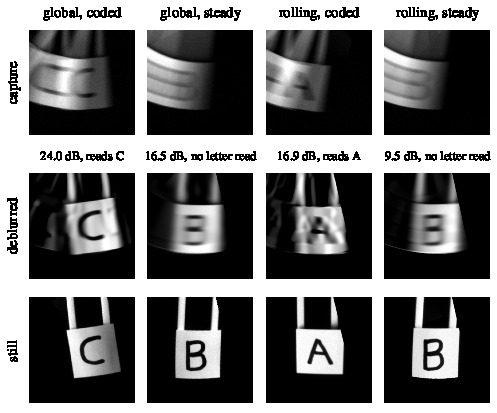
\includegraphics[width=\linewidth]{rig_cards}
  \caption{Coded light makes motion blur reversible, on the rig. The letter card on one blade of the fan
  turning at \SI{\rigCardSpeed}{rpm}, from the median capture (by PSNR) of each camera and light. Top: the
  capture, one exposure of 1.1 to \SI{1.4}{s}. Middle: our reconstruction, with its PSNR against the still
  and the letter a character reader finds in it. Bottom: a still of the stopped fan, turned onto the
  reconstructed blade. With coded light the letter comes back on both cameras, with some stripes left;
  with steady light of the same length it does not. Each panel is scaled to its own brightness.}
  \label{fig:rig-cards}
\end{figure}

 anything that moves forces a trade-off between blur and noise. A long exposure collects
enough light but smears the subject; a short one freezes it but is dark and noisy. Inspection of
rotating machinery, sport and traffic all suffer from this. Our test case is reading the letters on
the blades of a spinning fan, as one would read a marking on a rotating part without stopping it.

Ordinary motion blur cannot simply be undone. Under steady light a moving point traces a uniform
streak whose spectrum has exact zeros (\cref{fig:code}b), so detail at those frequencies is erased
and no algorithm can recover it. If the light is instead switched on and off in a well-chosen binary
code during the exposure, the blur keeps every frequency and becomes invertible~\cite{raskar2006coded}.

We build such a system with \emph{coded illumination}: a monitor beside the camera flashes the code
during one long exposure, so the camera needs no modification (\cref{fig:system}). The subject is a
fan with letters on its blades, driven by a stepper motor at a known speed. Unwrapping the image about
the hub turns the rotation into a shift, and the blur into a known linear operator that we invert
(\cref{fig:rig-cards}).

What is new is a three-way comparison of how the camera's shutter interacts with the code. A global
shutter exposes every row at once; a rolling shutter exposes row by row, so each row sees a different
part of the code. We reconstruct the rolling-shutter image with one blur for the whole frame or with
each row's own blur, and we also estimate the fan's speed from the photograph alone.

Our contributions are a coded illumination rig with a stepper-driven fan and both camera types
(\cref{sec:method}); an open reconstruction and speed estimation pipeline with automatic calibration;
and a measured comparison of coded against steady light on both cameras, with the three shutter
methods compared on the rig and in simulation, and a short exposure in simulation only
(\cref{sec:results}).



% Brief: very brief; academic papers only (no websites); say what we borrow or adapt.
% Keys are in refs.bib. Add a paper there before citing it.
\section{Related Work}
\label{sec:literature}

\paragraph{Coded exposure.}
Raskar et al.\ opened and closed a camera's shutter in a binary code during one exposure, turning
motion blur into an invertible operation~\cite{raskar2006coded}. Agrawal and Xu then chose codes
for both invertibility and for estimating the blur from the image~\cite{agrawal2009coded}. We borrow
the principle and the 52-bit code of~\cite{raskar2006coded}, but code the light instead of the
shutter.

\paragraph{Other ways to capture motion.}
Motion-invariant photography moves the camera so that the blur is the same for every
speed~\cite{levin2008motion}, and velocity-dependent codes adapt the code to the expected
speed~\cite{mccloskey2010velocity}. Both need a moving camera or prior knowledge of the speed; our
rig needs neither, and estimates the speed afterwards.

\paragraph{Rolling shutter.}
Reading a sensor row by row distorts moving objects~\cite{liang2008rolling}, and coded rolling
shutter photography exploits the row timing deliberately~\cite{gu2010coded}. We instead model each
row's own exposure window in the blur operator.

\paragraph{Reconstruction.}
We use Tikhonov-regularised least squares as a transparent baseline, and plug-and-play restoration
with a learned denoiser (DPIR)~\cite{zhang2022plug} as the main solver.

% Brief: approach + experimental setup + the relevant physics/maths (for a camera: the measurement
% model). System overview first, then subsystems.
\section{Method}
\label{sec:method}

\begin{figure}[t]
  \centering
  \placeholder{System photo with labels: monitor, fan with letter cards, matte black backing,
  camera, Raspberry Pi, Arduino + stepper driver. Inset: block diagram of signals and timing.}
  \caption{\TODO{The rig. Say what each part does and how far the camera is from the fan.}}
  \label{fig:system}
\end{figure}

\subsection{System overview}
\label{sec:overview}
The rig has three parts (\cref{fig:system}). An Arduino Uno drives a 28BYJ-48 stepper motor through a
ULN2003 driver, spinning a fan whose blades carry printed letters in front of a matte black backing.
A Raspberry Pi runs the camera and, on its own monitor facing the fan, shows a black/white code with
one bit per four \SI{60}{Hz} refreshes. One button in our capture software starts one long exposure
and the code together and saves the raw image with a log of when each bit was shown. Reconstruction
runs offline on a laptop. \TODO{Fan dimensions and camera distance.}

\subsection{Measurement model}
\label{sec:model}
After unwrapping the image to polar coordinates $(r,\theta)$ about the hub, a rotation at angular
speed $\omega$ is a shift along $\theta$. We discretise the exposure into short time steps $t_k$ of
length $\Delta t$. A polar sample $i$ on sensor line $\ell_i$ then records
\begin{equation}
  b_i = \sum_k w_k(\ell_i)\, x(\theta_i - \omega t_k) + n_i,
  \label{eq:forward}
\end{equation}
\begin{equation}
  w_k(\ell) = L(t_k)\,\bigl|[t_k - \tfrac{\Delta t}{2}, t_k + \tfrac{\Delta t}{2}) \cap [s_\ell, s_\ell + T)\bigr|,
  \label{eq:weights}
\end{equation}
where $x$ is the sharp image, $L(t)\in\{0,1\}$ the monitor brightness, $T$ the exposure, $s_\ell$ the
time line $\ell$ opens, and $n_i$ noise. Equation~\eqref{eq:forward} is linear in $x$, and with linear
interpolation in $\theta$ each ring of radius $r$ gives a sparse matrix,
$\mathbf{b}_r = \mathbf{A}_r(\omega)\,\mathbf{x}_r + \mathbf{n}_r$. Because the arc in view does not
wrap around, $\mathbf{x}_r$ extends beyond the window to hold light that moves into it during the
exposure.

The code decides whether $\mathbf{A}_r$ can be inverted. Under steady light the blur is a box whose
spectrum has exact zeros; a good code keeps every frequency well above zero (\cref{fig:code}).

\subsection{Global and rolling shutter}
\label{sec:shutters}

\begin{figure}[t]
  \centering
  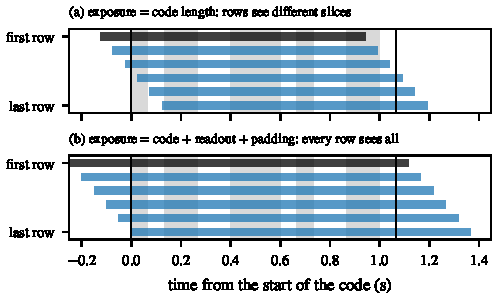
\includegraphics[width=\linewidth]{timing}
  \caption{When each sensor row collects light (bars) relative to the code (grey: monitor on), drawn
  for six rows with the readout four times longer than the rolling shutter camera's
  \SI{64}{ms} so that the stagger is visible. (a) With the exposure equal to the code, each row sees
  a different slice of the code, so one blur for the whole frame is wrong for most rows. (b) Our
  capture software lengthens the exposure by the readout time plus \SI{50}{ms}, so every row sees
  the whole code.}
  \label{fig:timing}
\end{figure}

The three methods differ only in $s_\ell$ in \eqref{eq:weights}. A global shutter opens every line
at once ($s_\ell = 0$). A rolling shutter opens line $\ell$ of $H$ at $s_\ell = \ell\,T_\mathrm{ro}/H$,
where $T_\mathrm{ro}$ is the readout time. \emph{Per row} uses each sample's own $s_\ell$;
\emph{per frame} uses the middle line's $s_\ell$ for every sample, as a pipeline that ignores the
rolling shutter would. \Cref{fig:timing}a shows why per frame then fails: the rows see different
slices of the code. Our capture software avoids this by construction (\cref{fig:timing}b): it
exposes for the code plus the readout plus \SI{50}{ms} of padding, so every row sees the full code
and the two rolling shutter methods coincide. We therefore compare them in simulation with the
exposure equal to the code, where they differ most.

\subsection{Reconstruction}
\label{sec:recon}
The baseline solves each ring by Tikhonov-regularised least squares with a first-difference
penalty $\mathbf{D}$,
\begin{equation}
  \hat{\mathbf{x}}_r = \arg\min_{\mathbf{x}} \|\mathbf{A}_r\mathbf{x}-\mathbf{b}_r\|_2^2
  + \lambda\|\mathbf{D}\mathbf{x}\|_2^2 .
  \label{eq:tikhonov}
\end{equation}
The main solver is DPIR~\cite{zhang2022plug}: half-quadratic splitting that alternates a data step
with a pretrained denoising network (DRUNet) acting as the prior, applied to all rings at once
through the block-diagonal operator. It needs no tuning. We scale the operator to unit gain and set
the noise level to six times a wavelet estimate from the polar data; the estimate reads about a
third of the true noise after resampling, and DPIR performed best at twice the true noise.

\subsection{Speed from a single photograph}
\label{sec:speed}
A wrong speed predicts the wrong blur, which DPIR cannot fit without breaking its prior. We therefore
reconstruct a band of 64 rings at 21 candidate speeds spanning $\pm20\%$ of the commanded speed, take
the data residual $\|\mathbf{A}(\omega)\hat{\mathbf{x}}(\omega)-\mathbf{b}\|_2$ at each, and refine the
minimum with a parabola through its neighbours. The same residual checks the direction of rotation:
if $-\omega$ fits better than $+\omega$ by a margin of 10\%, the sign is flipped.

\subsection{Calibration}
\label{sec:calibration}
The pipeline needs the hub centre, the radii of the blades and the arc they occupy. We find all
three from three photographs of the stopped fan, turned by a known number of motor steps between
them (\SI{4076}{} half-steps per revolution). For each pair of photographs we search for the centre
about which one rotates into the other, first on a coarse grid and then by Nelder-Mead; the median
over the pairs is the hub, and a spread above \SI{1}{px} warns that the camera moved. The code timing
comes from each capture's log, and a photograph of the stopped fan in the same setup is the
reference for image quality. \TODO{Measured hub spread on the rig: \X~px.}

\subsection{Experimental protocol}
\label{sec:protocol}

\begin{table}[t]
  \centering\small
  \caption{Rig and capture parameters. Readout times are the capture software's estimate (one over
  the sensor mode's maximum frame rate), logged with every capture. \TODO{Update the code if it is
  replaced (\cref{sec:limitations}).}}
  \label{tab:params}
  \begin{tabular}{@{}ll@{}}
    \toprule
    Parameter & Value \\
    \midrule
    Code & \rigBits~bits, \rigCodeMs~ms each, \rigCodeS~s \\
    Exposure & code + readout + \SI{0.05}{s} \\
    Global shutter camera & Sony IMX296, $1456\times1088$ \\
    Rolling shutter camera & OV5647, $2592\times1944$ \\
    Readout, global / rolling & 16.6 / \SI{64.0}{ms} \\
    Motor & 28BYJ-48, \SI{4076}{} half-steps/rev \\
    Fan speeds & \TODO{3, 5, 8, 10}~rpm \\
    Captures per condition & 10 \\
    Camera to fan & \X~cm \\
    \bottomrule
  \end{tabular}
\end{table}

\paragraph{Simulation.} Before the rig existed we validated the pipeline on renders. Blender renders
a single \SI{50}{mm} blade filling the frame height, hub above the frame, on a black background, at
$728\times544$~px in steps of \SI{8.3}{ms} while it turns at \SI{0.35}{rpm}; one scene carries
letters, a harder one a photograph plus letters. We apply the code and each line's exposure window
in software, then a sensor model with Poisson shot noise, a \SI{10000}{e^-} full well, \SI{3}{e^-}
read noise and a 10-bit converter, with steady light filling 70\% of the well on white. The code is
the 52-bit code of~\cite{raskar2006coded} at one bit per refresh (\SI{0.87}{s}). The short exposure
baseline is a single \SI{16.7}{ms} bit with $16\times$ analogue gain.

\paragraph{Rig.} \TODO{For each speed (\cref{tab:params}): 10 coded captures, 10 with steady light,
10 short exposures, and a reference photograph of the stopped fan in the same setup. Ground truth
speed from the step rate. Dark room.}

% Brief: qualitative results (including limitations) AND quantitative results compared against
% conventional/alternative approaches. At least one plot with axes, units and uncertainty.
% Pitch: every metric is mean +/- std over >= 10 captures per speed.
%
% Status: 5.1 and 5.3 are measured on the rig; 5.2 is simulation (pipeline validation, clearly labelled).
\section{Results}
\label{sec:results}

\subsection{The code and the monitor}
\label{sec:results-code}

\begin{figure}[t]
  \centering
  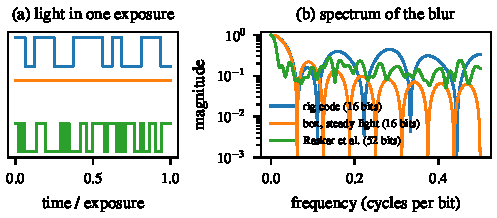
\includegraphics[width=\linewidth]{code_spectrum}
  \caption{(a) The monitor's brightness during one exposure for our rig's code, steady light, and
  the 52-bit code of Raskar et al.~\cite{raskar2006coded}. (b) The magnitude of each blur's spectrum
  (zero-padded DFT, 1 at zero frequency). Steady light has exact zeros, where detail is lost. The
  \rigBits-bit code used for every rig result never falls below \rigMinMTF, and the 52-bit code
  below \raskarMinMTF.}
  \label{fig:code}
\end{figure}

\begin{figure}[t]
  \centering
  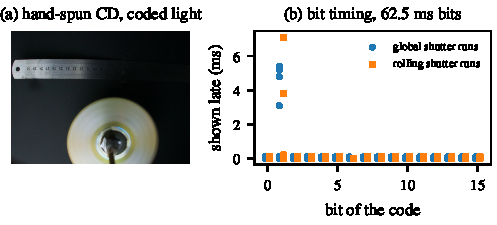
\includegraphics[width=\linewidth]{real_cd}
  \caption{First captures on the rig. (a) A hand-spun CD under coded light (global shutter, processed
  image). The speed varied during the exposure, so these captures cannot be deblurred.
  (b) How late each bit of the code was shown over all \realRuns~coded captures, from the display
  software's log: \realWithinOneMs~of \realBits~bits within \SI{1}{ms}, the worst \realMaxLateMs~ms
  (\realMaxLatePct\% of a bit), always bit \realLateBits.}
  \label{fig:real}
\end{figure}

\Cref{fig:code} compares the codes: steady light has exact spectral zeros, while the 52-bit code
of~\cite{raskar2006coded} keeps every frequency above \raskarMinMTF~of its zero-frequency value and
the \rigBits-bit rig code above \rigMinMTF, so neither loses detail outright. The monitor shows the
code on time: over \realRuns~captures, \realWithinOneMs~of \realBits~bits appeared within \SI{1}{ms}
of schedule (\cref{fig:real}b), the only late one being the first switch to black, at most
\realMaxLateMs~ms (\realMaxLatePct\% of a \realBitMs~ms bit). These times come from the display
software; measured optically (\cref{sec:calibration}), the screen brightens slowly, which the
pipeline models.

\subsection{Simulation: does the pipeline work?}
\label{sec:results-sim}

\begin{figure}[t]
  \centering
  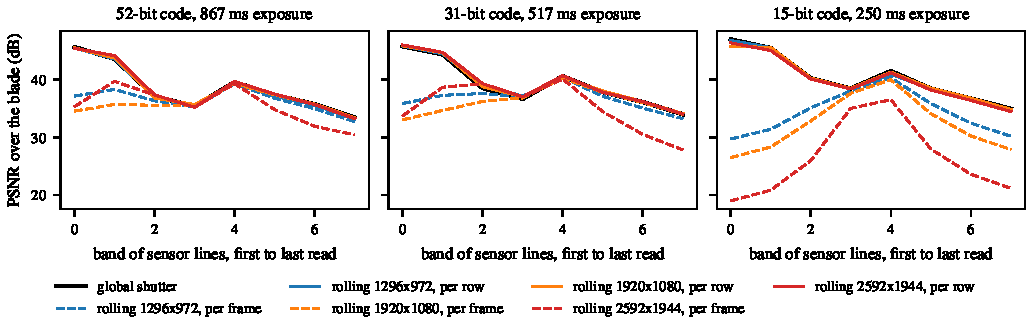
\includegraphics[width=\linewidth]{rows_axis0}
  \caption{Criterion 1 in simulation: image quality by band of sensor lines (first to last read),
  readout down the blade, with the shortest code, where per frame fails most. Black: global shutter;
  solid: per-row rolling shutter for three readout times; dashed: per frame, which falls away from the
  middle band it was timed for (mean \rowsShortFrameMeanA~dB, worst band \rowsShortFrameWorstA~dB,
  against \rowsShortRowMeanA~dB per row at the longest readout). Over all three codes and readouts,
  per row is within \rowsMaxMeanGapA~dB of the global shutter on average and \rowsMaxGapA~dB in its
  worst band. One noise draw per case.}
  \label{fig:rows}
\end{figure}

Simulation showed the pipeline works before any rig data existed. On the harder scene, a photograph
and letters on the blade, DPIR reconstructs the global shutter capture to \psnrGsTex~dB and the per-row
rolling shutter capture to \psnrRsRowTex~dB (\psnrRsFrameTex~dB per frame); steady light gives
\psnrConstTex~dB and a short exposure \psnrShortTex~dB (\cref{tab:solvers}).

\paragraph{Per row against per frame.}
\Cref{fig:rows} tests the first success criterion, per row within \SI{1}{dB} of the global shutter
in every band. Averaged over the frame it is met for every code and readout time; band by band it is
narrowly missed, by up to \rowsMaxGapA~dB in the first bands read, close to the noise of a single
draw. Per frame loses \rowsShortDropA~dB on average against the global shutter with a 15-bit code
and the full sensor readout. With the readout across the blade, per row is within
\rowsMaxMeanGapB~dB on average and \rowsMaxGapB~dB in its worst band.

\paragraph{When does coding pay?}
\Cref{tab:solvers} shows that coding the light pays when the blur is long. At \gainBlurOne~px of blur
steady light deblurs nearly as well (\gainSteadyFullOne~dB against \gainCodedFullOne~dB); at
\gainBlurThree~px coded light gives \gainCodedFullThree~dB against \gainSteadyFullThree~dB. A denoised short
exposure stays below coded light at every blur and light level in the table.

\begin{table}[t]
  \centering\small
  \caption{Simulation, global shutter, PSNR (dB) over the blade. Top: solvers on the two scenes.
  Bottom: coded light against steady light and a denoised short exposure as the blur (at the blade
  tip) grows, DPIR, at full light and at a tenth of the light; a separate noise draw from the top half.}
  \label{tab:solvers}
  % Tikhonov and DPIR: demo.py; the blur rows: coding_gain.py. Both via numbers.tex.
  \setlength{\tabcolsep}{4pt}
  \begin{tabular}{@{}lcc@{}}
    \toprule
    Solver & letters & photograph \\
    \midrule
    Tikhonov, best $\lambda$ & \tikGsLetters & \tikGsTex \\
    DPIR, no tuning & \psnrGsLetters & \psnrGsTex \\
    \midrule
    Blur (coded/steady/short) & full light & a tenth \\
    \midrule
    \gainBlurOne~px & \gainCodedFullOne~/ \gainSteadyFullOne~/ \gainShortFullOne
      & \gainCodedTenthOne~/ \gainSteadyTenthOne~/ \gainShortTenthOne \\
    \gainBlurTwo~px & \gainCodedFullTwo~/ \gainSteadyFullTwo~/ \gainShortFullTwo
      & \gainCodedTenthTwo~/ \gainSteadyTenthTwo~/ \gainShortTenthTwo \\
    \gainBlurThree~px & \gainCodedFullThree~/ \gainSteadyFullThree~/ \gainShortFullThree
      & \gainCodedTenthThree~/ \gainSteadyTenthThree~/ \gainShortTenthThree \\
    \bottomrule
  \end{tabular}
\end{table}

\paragraph{Speed from the photograph.}
The data residual is lowest near the true speed: the estimate is within
\speedErrLetters\% and \speedErrTex\% on the two scenes, against the 5\% target.

\subsection{Rig results}
\label{sec:results-rig}
Every capture was deblurred, none was skipped, and the direction check never flipped a sign.
\Cref{fig:rig-cards} shows the median capture of each set at \SI{\rigCardSpeed}{rpm}. PSNR is
against a still of the stopped fan with the static scene taken out of both (\cref{sec:calibration}),
on the blade picked from the whole capture (margins of at least \rigMarginMin~and \rigRsMarginMin).
With the global shutter camera, coded light deblurs to \rigCodedThree, \rigCodedFive~and
\rigCodedEight~dB at 3, 5 and \SI{8}{rpm}, against \rigSteadyThree, \rigSteadyFive~and
\rigSteadyEight~dB for steady light of the same length deblurred by the same solver: \rigGapMin~to
\rigGapMax~dB better at every speed, by more than the spread between captures
(\cref{fig:rig-psnr}). The rolling shutter camera scores lower, \rigRsCodedThree,
\rigRsCodedFive~and \rigRsCodedEight~dB, but coded light again leads steady light, by \rigRsGapMin~to
\rigRsGapMax~dB. An earlier global shutter session at \SI{3}{rpm} (\rigOctTwentySix~$\pm$ \rigOctTwentySixSd~dB) is
left out: its blades could barely be told apart (margins down to \rigOctTwentySixMarginMin).

\begin{figure}[t]
  \centering
  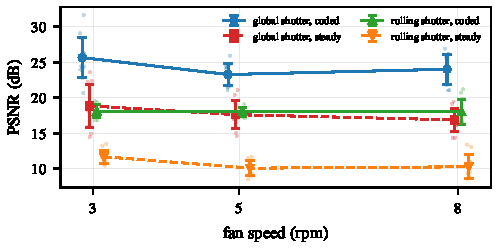
\includegraphics[width=\linewidth]{rig_psnr}
  \caption{The rig: PSNR of the deblurred blades against the stopped fan, coded and steady light of the
  same length, both deblurred with the same solver and monitor model, on both cameras (rolling shutter
  per row). Bars: mean $\pm$ std over 9 to 12 captures; dots: each capture.}
  \label{fig:rig-psnr}
\end{figure}

\paragraph{Criterion 1: per row against the global shutter.} On the rig, per row and per frame gave
identical numbers on all 18 captures run both ways: the padded exposure lets every row see the whole
code (\cref{fig:timing}b), so the per-frame loss of \cref{fig:rows} cannot occur. Band by band the
rolling shutter camera is \rigBandGapMin~to \rigBandGapMax~dB below the global shutter camera
(\rigBandGapMean~dB on average, \cref{fig:rig-rows}), so the \SI{1}{dB} target is missed on the rig.
This compares two cameras, not two corrections: different sensors and lenses, and a blade 1.6 times
larger in the frame, so the same motion smears it over 1.6 times as many pixels.

\begin{figure}[t]
  \centering
  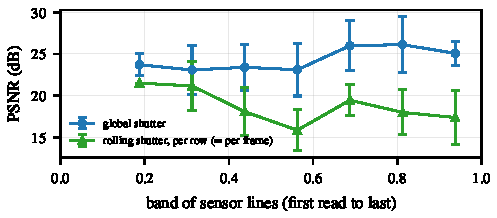
\includegraphics[width=\linewidth]{rig_rows}
  \caption{Criterion 1 on the rig, coded light, every speed: PSNR by band of sensor lines, first read
  to last, mean $\pm$ std over the captures whose blade reached the band. Rolling shutter per row and per
  frame give identical numbers here (padded exposure).}
  \label{fig:rig-rows}
\end{figure}

\paragraph{Criterion 2: letters read.} The still's card read as one of the fan's three letters in
all \rigCardsAll~global and \rigRsCardsAll~rolling shutter captures, and no letter was read from any
capture before deblurring. After deblurring, the global shutter camera read \rigReadCodedThree,
\rigReadCodedFive~and \rigReadCodedEight\% of the letters with coded light at 3, 5 and \SI{8}{rpm},
against \rigReadSteadyThree, \rigReadSteadyFive~and \rigReadSteadyEight\% with steady light
(\cref{fig:rig-criteria}a). The target, at least 90\% with coded light where steady light gives under
50\%, is met at \SI{8}{rpm}; at 3 and \SI{5}{rpm} steady light is still legible. The rolling shutter
camera also reads more with coded light at every speed, but falls short of 90\% at 5 and \SI{8}{rpm}
(\rigReadRsCodedFive~and \rigReadRsCodedEight\%).

\paragraph{Criterion 3: speed from the blur.} With coded light the speed from the blur is within 5\%
of the commanded speed on \rigSpeedWithinCoded~of \rigSpeedAllCoded~global and
\rigSpeedWithinRsCoded~of \rigSpeedAllRsCoded~rolling shutter captures (\cref{fig:rig-criteria}b).
Steady light, whose blur is nearly a plain box, does worse: \rigSpeedWithinSteady~of
\rigSpeedAllSteady~and \rigSpeedWithinRsSteady~of \rigSpeedAllRsSteady~within 5\%.

\begin{figure}[t]
  \centering
  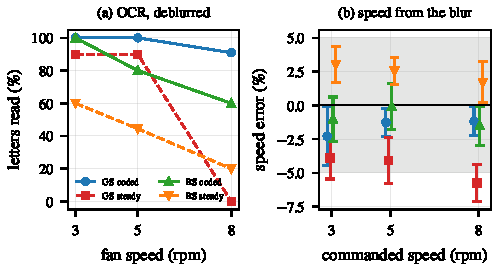
\includegraphics[width=\linewidth]{rig_criteria}
  \caption{The rig, both cameras (GS global, RS rolling shutter). (a) Criterion 2: letters read by OCR
  after deblurring, against the same card on the still. (b) Criterion 3: speed from the blur against the
  commanded speed, mean $\pm$ std; shaded: the $\pm5\%$ target.}
  \label{fig:rig-criteria}
\end{figure}



% Brief: what didn't work and why, especially fundamental limits.
\section{Limitations and Pitfalls}
\label{sec:limitations}

\begin{table}[t]
  \centering\small
  \caption{What goes wrong, simulated at the rig's scale: a three-blade fan with a text card on each
  blade, global shutter, the rig's code, \SI{5}{rpm}, run through the same commands as the lab.
  PSNR against the stopped fan over three captures.}
  \label{tab:faults}
  % Source: software/deconvolution/STUDIES.md, "Rig-scale stress test".
  \begin{tabular}{@{}lc@{}}
    \toprule
    Case & PSNR (dB) \\
    \midrule
    Baseline & 32.9 to 33.4 \\
    Fan at 10 / \SI{15}{rpm} & 29.6 to 30.2 / 22.4 \\
    5\% room light & 30.9 to 31.2 \\
    White stand behind the blades & 8.3 to 11.0 \\
    One bit shown twice as long & 19.6 \\
    Speed given with the wrong sign & 15.8 \\
    \quad the same, with the direction check & 32.95 \\
    \bottomrule
  \end{tabular}
\end{table}

\paragraph{The subject must turn at a known, steady speed.}
Our first captures used a CD spun by hand (\cref{fig:real}a). The speed changed during each
exposure, so no single blur explained the image and none could be deblurred. This is why the rig
uses a stepper motor. In simulation, a speed error of 1, 2 and 5\% costs 0.8, 2.7 and \SI{8.5}{dB};
the stepper's nominal 4096 steps per revolution against the true 4076 alone makes the fan 0.5\%
fast, which the speed search (\cref{sec:speed}) corrects. % STUDIES.md, fault costs
\TODO{Measured speed ripple of the stepper, if any.}

\paragraph{The background must be dark.}
Anything bright behind the blades is blurred by the code too, and is not in the model. A white
stand behind the fan drops the reconstruction to about \SI{10}{dB} (\cref{tab:faults}), so the rig
uses a matte black backing in a dark room.

\paragraph{The current rig code has spectral zeros.}
The \rigBits-bit code on the rig loses detail at multiples of $1/9$ cycle per bit
(\cref{fig:code}b), like steady light. DPIR's prior hides much of the loss in simulation, but the
loss is fundamental. \TODO{Swap for a code without zeros (e.g.\ the 52-bit code, or a searched
16-bit code) and state which one the rig results use.}

\paragraph{Speed, light and timing.}
Above about \SI{10}{rpm} the blades smear into each other and quality falls quickly
(\cref{tab:faults}). The speed search needs a guess within 20\%, as the residual flattens far from
the truth (\cref{fig:speed}). A dropped or repeated bit costs about \SI{6}{dB} at blade scale, and the
monitor's first switch to black ran up to \realMaxLateMs~ms late (\cref{fig:real}b).
% STUDIES.md, fault costs: one bit shown twice, the next skipped: -6.1 dB

\paragraph{Cost.}
Each reconstruction takes seconds and under \SI{1}{GB} at 10~px/mm, but memory grows roughly with
the cube of the resolution, so very fine sampling is out of reach on a laptop.
% STUDIES.md: 7 s and 0.8 GB at 10 px/mm, 44 s and 5.2 GB at 40 px/mm (2.8 rpm, 40-50 mm blades)

\TODO{Anything else found in the lab.}

% Brief: summarise, and what we would do with another 2 months.
\section{Conclusions and Future Work}
\label{sec:conclusion}

We built a coded illumination rig that turns an ordinary camera and monitor into a flutter shutter
camera, and a pipeline that reverses the blur and recovers the speed of a spinning fan from a
single photograph. In simulation the reconstruction reaches \psnrGsTex~dB on a textured blade, per-row
rolling shutter matches the global shutter to within \rowsMaxMeanGapA~dB on average, and the speed is recovered to
within \speedErrTex\%. On the rig, the monitor shows the code to within \SI{1}{ms} for
\realWithinOneMs~of \realBits~bits. \TODO{Rig results against each success criterion.}

With two more months we would replace the monitor with an LED, whose microsecond switching would
allow codes hundreds of bits long; design codes for the rolling shutter, so that its row timing adds
information instead of being corrected for; drive the motor continuously and measure its speed
independently; and move from a fan to everyday moving scenes, where the motion must be estimated
for every object.


\bibliographystyle{IEEEtran}
\bibliography{refs}



\ifpeerreview \else
%%%% For the camera ready version, please fill out this
%%%% biography. Your camera ready should be within a 12 page limit
%%%% including acknowledgments, references and biography.

% If you have an EPS/PDF photo (graphicx package needed) extra braces are
% needed around the contents of the optional argument to biography to prevent
% the LaTeX parser from getting confused when it sees the complicated
% \includegraphics command within an optional argument. (You could
% create your own custom macro containing the \includegraphics command
% to make things simpler here.)
% \begin{IEEEbiography}[{\includegraphics[width=1in,height=1.25in,clip,keepaspectratio]{mshell}}]{Michael Shell}
% or if you just want to reserve a space for a photo:

% insert where needed to balance the two columns on the last page with
% biographies
%\newpage

% if you will not have a photo at all:

% You can push biographies down or up by placing
% a \vfill before or after them. The appropriate
% use of \vfill depends on what kind of text is
% on the last page and whether or not the columns
% are being equalized.
%\vfill

\fi

\end{document}


